\documentclass[a4paper, 11pt]{article}
\usepackage{fullpage}
\usepackage{mathtools, nccmath}
\usepackage{graphicx}
\usepackage{float}
\usepackage{amsmath}
\usepackage{caption}
\renewcommand{\figurename}{Fig.}
\renewcommand{\refname}{Bibliografia}

\begin{document}
% Header
\noindent
\large\textbf{Corso di Metodi di Ottimizzazione} \hfill \textbf{Gruppo E} \\
\normalsize A.A. 2018/2019 \hfill Ing. Saverio Del Prete \\
Prof. Raffaele Martone \hfill Ing. Bernardo Giordano \\
\hphantom{}\hfill Ing. Lucia Migliaccio

\section*{Traccia del problema}

Progetto ottimo di un campo magnetico con incognite geometriche e di corrente di
una spira.

\section*{Descrizione del sistema fisico}

Il sistema è composto da un certo numero di spire simmetriche (supporremo $n=6$)
concentriche rispetto allo stesso asse $z$. I parametri di progetto, ovvero
posizione, raggio e intensità di corrente, sono noti per tutte le spire tranne
che per una coppia. Le correnti sono concordi per tutte le spire. 

\begin{figure}[H]
    \centering
    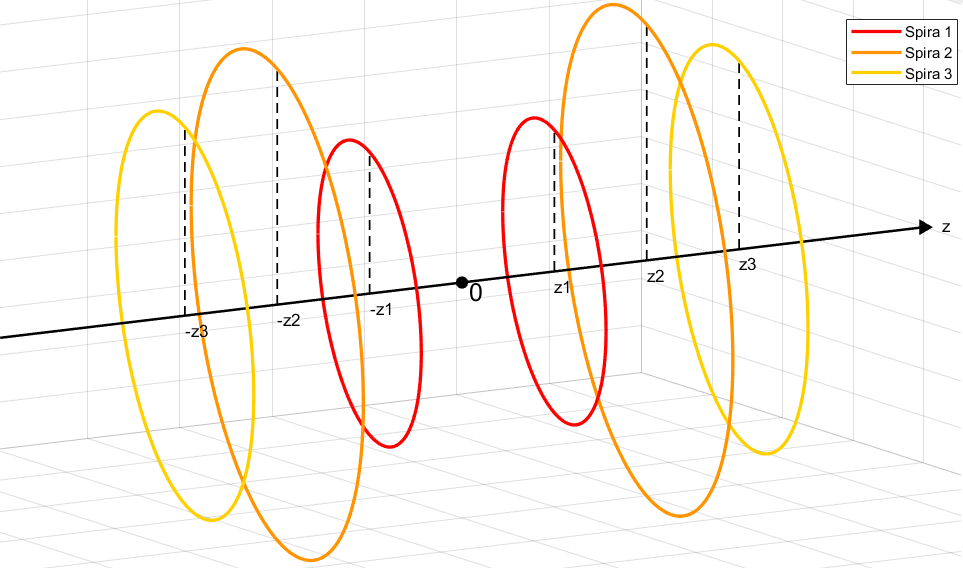
\includegraphics[width=12cm]{assets/figure1}
    \caption{Schematizzazione del sistema fisico.}
\end{figure}

\noindent
Il campo magnetico generato dalla corrente circolante nelle spire può essere
valutato sull’asse utilizzando la legge di Biot-Savart. La legge di Biot-Savart
permette di valutare il campo magnetico B prodotto in un punto dello spazio da
una spira percorsa da corrente elettrica. \\ \\
\noindent
Il campo magnetico sull’asse $z$  di una spira caratterizzata da una corrente
$I$, lunghezza $L$, raggio $R$ e posizione $Z$ si valuta come
\[dB_{z}=\frac{\mu_{0}IdL}{4\pi}\frac{R}{\left((Z{\pm}z)^{2}+R^{2}\right)^{3/2}}\]
dove $\mu_{0}$ è la permeabilità magnetica nel vuoto, $\mu_{0}=4{\pi}10^{-7}
H/m$. \\
L’integrale di $dL$ risulta essere proprio la circonferenza della spira, ovvero
$2{\pi}R$. Integrando quindi, si ricava la funzione del campo magnetico
sull'asse
\[B_{z}=\frac{\mu_{0}}{4\pi}\frac{2{\pi}R^{2}I}{\left((Z{\pm}z)^{2}+R^{2}\right)^{3/2}}=\frac{\mu_{0}}{2}\frac{R^{2}I}{\left((Z{\pm}z)^{2}+R^{2}\right)^{3/2}}\]
Siano $Z_{i}$, $R_{i}$ e $I_{i}$ rispettivamente la posizione, il raggio e la
corrente relative alla spira $i$-esima. \\
Sia inoltre $n=6$ il numero complessivo delle spire facenti parte del sistema.
Considerando adesso la sovrapposizione degli effetti di tutte le spire del
sistema e tenendo presente che le spire sono simmetriche rispetto al piano
$r{\theta}$, il campo magnetico complessivo sull’asse $z$ sarà:

\begin{align*}
    B_{z}
    &=\frac{\mu_{0}}{4{\pi}}\left(\sum_{i=1}^{n}\frac{2{\pi}I_{i}R_{i}^{2}}{\left(\left(Z_{i}-z\right)^{2}+R_{i}^{2}\right)^{3/2}}+\frac{2{\pi}I_{i}R_{i}^{2}}{\left(\left(Z_{i}+z\right)^{2}+R_{i}^{2}\right)^{3/2}}\right)\\
    &=\frac{\mu_{0}}{2}\left(\sum_{i=1}^{n}\frac{I_{i}R_{i}^{2}}{\left(\left(Z_{i}-z\right)^{2}+R_{i}^{2}\right)^{3/2}}+\frac{I_{i}R_{i}^{2}}{\left(\left(Z_{i}+z\right)^{2}+R_{i}^{2}\right)^{3/2}}\right)
\end{align*}

\noindent
L'obiettivo del progetto della spira mancante risulta essere la migliore
approssimazione di un campo magnetico avente la seguente caratteristica:

\begin{figure}[H]
    \centering
    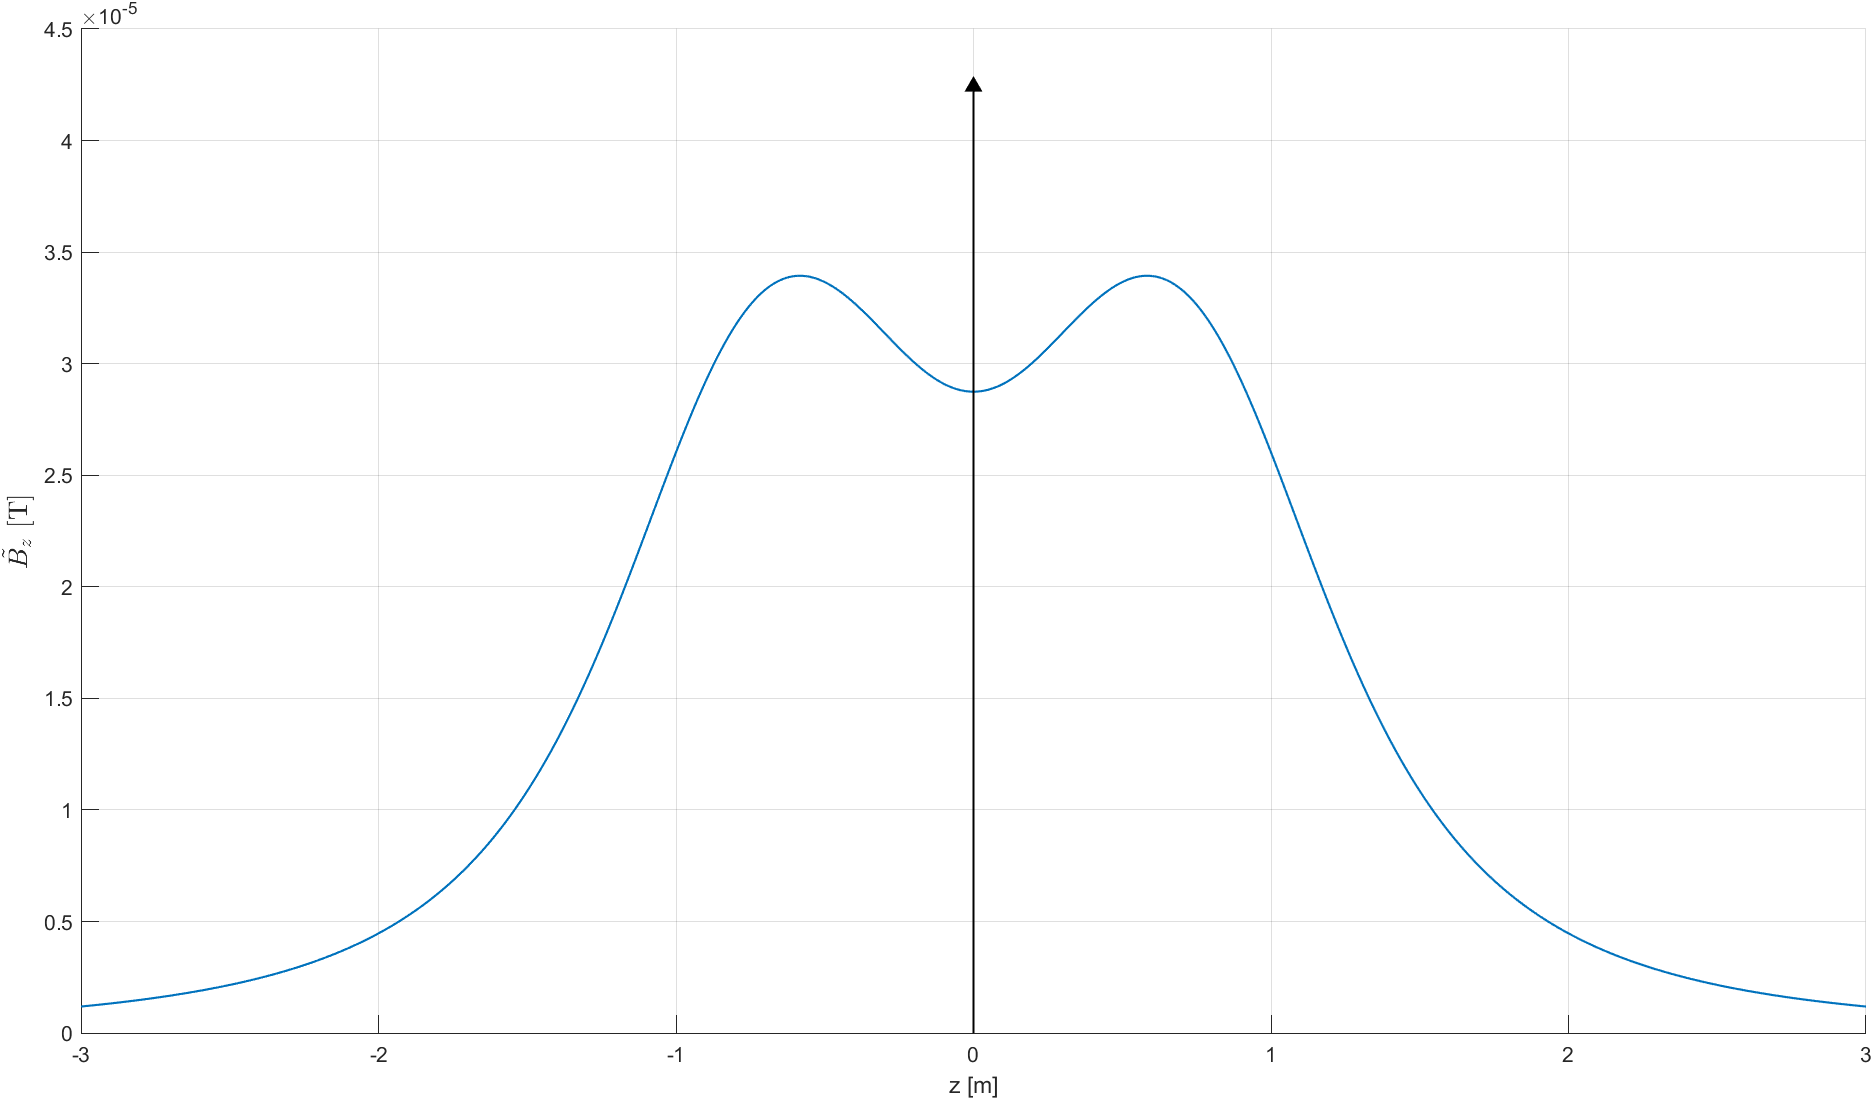
\includegraphics[width=16cm]{assets/figure2}
    \caption{Campo magnetico sull'asse $z$ desiderato.}
\end{figure}
\noindent
Sia adesso $B_{z}$ il campo magnetico generato dalla sovrapposizione delle spire
del sistema, e $\tilde{B_{z}}$ il campo magnetico desiderato. Al fine di
ottenere una discrepanza più piccola possibile, è di particolare interesse lo
studio del minimo della funzione
\[||B_{z}-\tilde{B_{z}}||\] Siccome i parametri di progetto delle spire 1 e 3
del sistema (e, quindi, delle rispettive spire simmetriche) sono noti ed
esattamente uguali a quelli del sistema desiderato, la suddetta differenza in
norma si scriverà come:

\begin{equation}
    \begin{split}
        ||B_{z_{2}}-\tilde{B_{z_{2}}}||
        =& \Bigl|\Bigl|\frac{\mu_{0}}{2}(\frac{I_{2}R_{2}^{2}}{((Z_{2}-z)^{2}+R_{2}^{2})^{3/2}}+\frac{I_{2}R_{2}^{2}}{((Z_{2}+z)^{2}+R_{2}^{2})^{3/2}})+ \\
         & -\frac{\mu_{0}}{2}(\frac{\tilde{I_{2}}\tilde{R_{2}}^{2}}{((\tilde{Z_{2}}-z)^{2}+\tilde{R_{2}}^{2})^{3/2}}-\frac{\tilde{I_{2}}\tilde{R_{2}}^{2}}{((\tilde{Z_{2}}+z)^{2}+\tilde{R_{2}}^{2})^{3/2}})\Bigr|\Bigr| \\
        =& \frac{\mu_{0}}{2}\Bigl|\Bigl|\frac{I_{2}R_{2}^{2}}{((Z_{2}-z)^{2}+R_{2}^{2})^{3/2}}+\frac{I_{2}R_{2}^{2}}{((Z_{2}+z)^{2}+R_{2}^{2})^{3/2}}+ \\
         & -\frac{\tilde{I_{2}}\tilde{R_{2}}^{2}}{((\tilde{Z_{2}}-z)^{2}+\tilde{R_{2}}^{2})^{3/2}}-\frac{\tilde{I_{2}}\tilde{R_{2}}^{2}}{((\tilde{Z_{2}}+z)^{2}+\tilde{R_{2}}^{2})^{3/2}}\Bigr|\Bigr|
    \end{split} 
\end{equation}
\noindent

\section*{Campionamento e normalizzazione}

Prima di poter definire la funzione obiettivo ed effettuarne un'analisi
numerica, è necessario applicare due tecniche: campionamento e normalizzazione.
\\
Il campionamento è una tecnica che consiste nel discretizzare una funzione
continua nel tempo. L'ampiezza del passo di campionamento può essere valutato a
intervalli temporali regolari e non. \\
In questo caso specifico, si è deciso di utilizzare un campionamento a passo
costante. \\
La normalizzazione è l'operazione la quale, dato un vettore, lo si porta ad
avere una norma unitaria. \\
% aggiungere altre cose sulla normalizzazione
La funzione verrà campionata su $N_{p}$ valori dell'asse $z$. La funzione
campionata, inoltre, verrà normalizzata e mediata sul valor medio di
$\tilde{B_{z}}$, in modo tale da esprimere la funzione obiettivo come
percentuale di scostamento tra il campo magnetico progettato e quello ideale. \\
Campionando e normalizzando la (1), la \emph{funzione obiettivo} si scriverà
come:
 
\begin{equation}
    \begin{split}
        F_{obj}(I_{2},R_{2},Z_{2}) =
        & \frac{1}{{\tiny <} \tilde{B_{z}}{\tiny >}} \Biggl[ \frac{1}{Np} \sum\limits_{k=1}^{Np} \Bigl|\Bigl|\frac{I_{2}R_{2}^{2}}{((Z_{2}-z_{k})^{2}+R_{2}^{2})^{3/2}}+\frac{I_{2}R_{2}^{2}}{((Z_{2}+z_{k})^{2}+R_{2}^{2})^{3/2}}+ \\
        & -\frac{\tilde{I_{2}}\tilde{R_{2}}^{2}}{((\tilde{Z_{2}}-z_{k})^{2}+\tilde{R_{2}}^{2})^{3/2}}-\frac{\tilde{I_{2}}\tilde{R_{2}}^{2}}{((\tilde{Z_{2}}+z_{k})^{2}+\tilde{R_{2}}^{2})^{3/2}}\Bigr|\Bigr|^{2}\biggr]^{\!1/2}
    \end{split} 
\end{equation}
\noindent

\section* {Ricerca del minimo}

L'algoritmo di ricerca del minimo fa uso del concetto di simplesso, cioè un
politopo di $N+1$ vertici in $N$ dimensioni, vale a dire: un segmento in una
dimensione, un triangolo in due dimensioni, un tetraedro in tre dimensioni, e
così via. Il metodo permette di limitare la ricerca della soluzione ottima ai
vertici del politopo. \\
La ricerca avviene attraverso il movimento del politopo, il quale può:

\begin{itemize}
\item \textbf{Ribaltarsi}: si valuta la funzione negli $N$ vertici del
simplesso, individuando qual è il vertice nel quale la funzione assume il valore
\emph{peggiore} (nel caso di un problema di ricerca del minimo, il caso peggiore
è quello in cui la funzione assume valore più grande tra tutti i vertici del
simplesso considerato). Una volta identificato il vertice peggiore, il simplesso
si ribalta rispetto a quest'ultimo, tenendo fermi gli altri $N-1$ vertici. \\
L'algoritmo può però ritrovarsi in una situazione di loop, dove il vertice
peggiore risulta essere proprio l'ultimo rispetto al quale è stato effettuato il
ribaltamento. In questo caso, si ribalta rispetto al \emph{secondo peggior
vertice}. 
\item \textbf{Contrarsi}: se un vertice del politopo \emph{vive} più a lungo di
un numero arbitrario di iterazioni $M$, il politopo viene contratto, dimezzando
i lati dell'ultimo simplesso tenendo fermo il vertice \emph{migliore}.
\end{itemize}

\noindent
L'algoritmo di ricerca del minimo mediante l'uso del politopo è un metodo di
\emph{ordine 0}, ovvero non richiede l'uso delle derivate, nonostante riesca a
stimare una direzione di discesa della funzione obiettivo.

\section*{Implementazione dell'algoritmo}

L'algoritmo implementato per la soluzione del problema della ricerca del minimo
consiste in una fase di \emph{inizializzazione}, una di \emph{loop} (nella quale
vengono effettuate tutte le operazioni di ribaltamento e contrazione del
simplesso) e una di \emph{controllo delle condizioni di arresto} del loop. \\ \\
La fase di inizializzazione consiste nell'impostazione di tutte le variabili
necessarie al funzionamento dell'algoritmo, che per design vengono
parametrizzate, in modo tale da rendere comodo l'utilizzo dell'algoritmo in
differenti condizioni iniziali, tra cui:
\begin{itemize}
\item \textbf{Passo di campionamento}, necessario all'approssimazione più o meno
grossolana della funzione obiettivo da studiare.
\item \textbf{Range dei parametri liberi}, con i quali si stabiliscono due
valori limite che dovranno essere rispettati da tutte le variabili da
ottimizzare.
\item \textbf{Condizioni di arresto}, necessarie per stabilire fino a quanto
l'algoritmo dovrà iterare per garantire dei risultati soddisfacenti. Tra le
innumerevoli condizioni possibili, verranno considerate il \emph{massimo numero
di ribaltamenti}, un valore di \emph{massimo errore percentuale} rispetto alla
funzione desiderata e un vincolo sulla \emph{minima lunghezza del lato} del
simplesso generato ad ogni passi.
\item \textbf{Punto iniziale}, che condizionerà, insieme all'andamento della
funzione, la generazione di determinati simplessi piuttosto che altri.
\end{itemize}

\noindent
Una volta parametrizzate le condizioni iniziali, l'algoritmo entrerà in fase di
loop, dove eseguirà ripetutamente le seguenti operazioni:

\begin{enumerate}
\item Un simplesso iniziale $s$ con centroide in $s_{0}$ viene aggiunto ad un
array di simplessi $polytope$
\item Controllo se un vertice di $s = polytope(end)$ ha vissuto per $k$
iterazioni
\item Se si:
\begin{enumerate}
\item Trovo il vertice $i$ di $s$ dove $F_{obj}$ assume valore minore
\item Dimezzo la lunghezza dei lati di $s$ lasciando fermo il vertice $i$,
ottenendo $s_{new}$
\end{enumerate}
\item Se no:
\begin{enumerate}
\item Trovo il vertice $i$ di $s$ dove $F_{obj}$ assume valore massimo
\item Ribalto $s$ tenendo fermi i vertici $k \ne i$, ottenendo $s_{new}$
\item Se $F_{obj}(s(i)) \leq F_{obj}(s_{new}(i))$:
\begin{enumerate}
\item Trovo il secondo vertice $j$ di $s$ dove $F_{obj}$ assume valore massimo
\item Ribalto $s$ tenendo fermi i vertici $k \ne j$, ottenendo $s_{new}$
\end{enumerate}
\end{enumerate}
\item Aggiungo $s_{new}$ a $polytope$, $polytope(end+1) = s_{new}$
\item Interrompi se almeno una condizione di arresto è verificata, altrimenti
ripeti dal passo 2.
\end{enumerate}

\noindent
L'algoritmo può essere schematizzato in maniera compatta secondo il seguente
diagramma di flusso:

\begin{figure}[H]
    \centering
     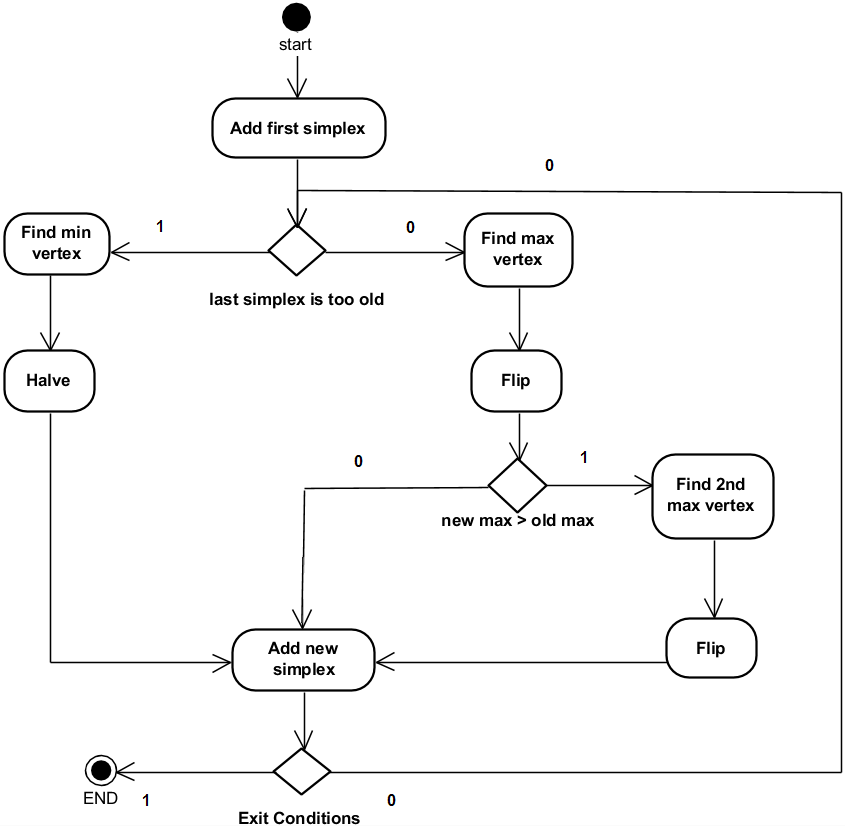
\includegraphics[width=14cm]{assets/figure3}
     \caption{Diagramma di flusso dell'algoritmo del simplesso.}
\end{figure}
\noindent

\section*{Scelta dei parametri}

Al fine di avvicinarci alla caratteristica descritta in $Fig. 2$, vanno scelti
opportunamente il valore dei raggi, delle correnti e delle posizioni relative a
tutte le spire, comprese quelle da progettare (spire 2 e 4). \\ \\
\centerline{ \textbf{Spira 1}: $R_{1}$ = 0.7m \\ $I_{1}$ = 3 A \\ $Z_{1}$ = -0.4m} 
\centerline{ \textbf{Spira 2}: $R_{2}$ = 0.8m \\ $I_{2}$ = 5 A \\ $Z_{2}$ = -0.7m}
\centerline{ \textbf{Spira 3}: $R_{3}$ = 0.6m \\ $I_{3}$ = 2 A \\ $Z_{3}$ = -0.9m}
\centerline{ \textbf{Spira 4}: $R_{4}$ = 0.7m \\ $I_{4}$ = 3 A \\ $Z_{4}$ = 0.4m}
\centerline{ \textbf{Spira 5}: $R_{5}$ = 0.8m \\ $I_{5}$ = 5 A \\ $Z_{5}$ = 0.7m}
\centerline{ \textbf{Spira 6}: $R_{6}$ = 0.6m \\ $I_{6}$ = 2 A \\ $Z_{6}$ = 0.9m}
\\ \\
\noindent
Si terrà inoltre considerazione di un campionamento a passo costante e di un
range di campionamento dell'asse $z$ che si estenderà fino a circa 3 volte oltre
la posizione dell'ultima spira. Siccome la spira più lontana dal centro di
simmetria è posta in $z = 0.9 m$, l'asse $z$ verrà campionato per $-3 m \le z
\le 3 m$. \\
Limiteremo a priori, inoltre, il massimo raggio e la massima posizione della
spira da progettare, in modo tale che entrambe non superino $1 m$.

\section*{Esperimenti}
\section{Minimo in 2 dimensioni senza vincoli}

Il primo test effettuato è stata la ricerca del minimo con due gradi di libertà,
supponendo che la variabile $Z = 0.7m$ sia fissata. Il test sarà ripetuto in due
diverse condizioni iniziali, in modo tale da poter apprezzare la differenza
nell'errore percentuale al variare del numero di campioni e della percentuale
minima di errore ammessa. \\
Come si evince dalle tabelle, i risultati sono più soddisfacenti con un maggior
numero di campioni.

\begin{table}[h]
    \caption{Test 1}
    \begin{center}
    \begin{tabular}{|l|l|l|l|} 
    \hline 
Gradi di libertà & \textbf{2} &  &  \\ \hline 
Passo & \textbf{0.1000} & Campioni & \textbf{61} \\ \hline 
Punto di minimo & \textbf{{[}5.000 0.800{]}} & Punto di minimo &
\textbf{{[}4.986 0.793{]}} \\ \hline 
Punto iniziale & \textbf{{[}3.000 0.300{]}} & Fobj nel punto & \textbf{0.00478}
\\ \hline 
Lunghezza iniziale & \textbf{0.300} & Dimezzamenti & \textbf{4} \\ \hline 
Lunghezza minima & \textbf{0.00100} & Lunghezza finale & \textbf{0.032} \\
\hline
Flip massimi & \textbf{1000} & Flips & \textbf{55} \\ \hline 
Tolleranza & \textbf{1.000\%} & \textbf{Perc. di errore} & \textbf{0.478\%} \\
\hline 
    \end{tabular}
    \end{center}
    \end{table}

    \begin{table}[h]
        \caption{Test}
        \begin{center}
        \begin{tabular}{|l|l|l|l|} 
        \hline
        \multicolumn{2}{|c|}{Parametri in ingresso} & \multicolumn{2}{c|}{Valori in uscita} \\ \hline
        Gradi di libertà  & \textbf{2} &  &  \\ \hline 
        Passo & \textbf{0.1000} & Campioni & \textbf{61} \\ \hline 
        Punto di minimo & \textbf{{[}5.000 0.800{]}} & Punto di minimo & \textbf{{[}4.986 0.793{]}} \\ \hline 
        Punto iniziale & \textbf{{[}3.000 0.300{]}} & Fobj nel punto & \textbf{0.00478} \\ \hline 
        Lunghezza iniziale & \textbf{0.300} & Dimezzamenti & \textbf{4} \\ \hline 
        Lunghezza minima & \textbf{0.00001} & Lunghezza finale & \textbf{0.0325} \\ \hline
        Flip massimi & \textbf{1000} & Flips & \textbf{55} \\ \hline 
        Tolleranza & \textbf{1.000\%} & \textbf{Perc. di errore} & \textbf{0.478\%} \\ \hline 
        \end{tabular} 
        \end{center}
        \end{table}
    

\begin{table}[h]
    \caption{Test 2}
    \begin{center}
    \begin{tabular}{|l|l|l|l|} 
    \hline 
Gradi di libertà & \textbf{2} &  &  \\ \hline 
Passo & \textbf{0.0100} & Campioni & \textbf{601} \\ \hline 
Punto di minimo & \textbf{{[}5.000 0.800{]}} & Punto di minimo &
\textbf{{[}4.998 0.800{]}} \\ \hline 
Punto iniziale & \textbf{{[}3.000 0.300{]}} & Fobj nel punto & \textbf{0.000560}
\\ \hline 
Lunghezza iniziale & \textbf{0.300} & Dimezzamenti & \textbf{7} \\ \hline 
Lunghezza minima & \textbf{0.00100} & Lunghezza finale & \textbf{0.00406} \\
\hline
Flip massimi & \textbf{1000} & Flips & \textbf{90} \\ \hline 
Tolleranza & \textbf{0.100\%} & \textbf{Perc. di errore} & \textbf{0.0563\%} \\
\hline 
    \end{tabular} 
    \end{center}
    \end{table}

\begin{figure}[H]
    \centering
        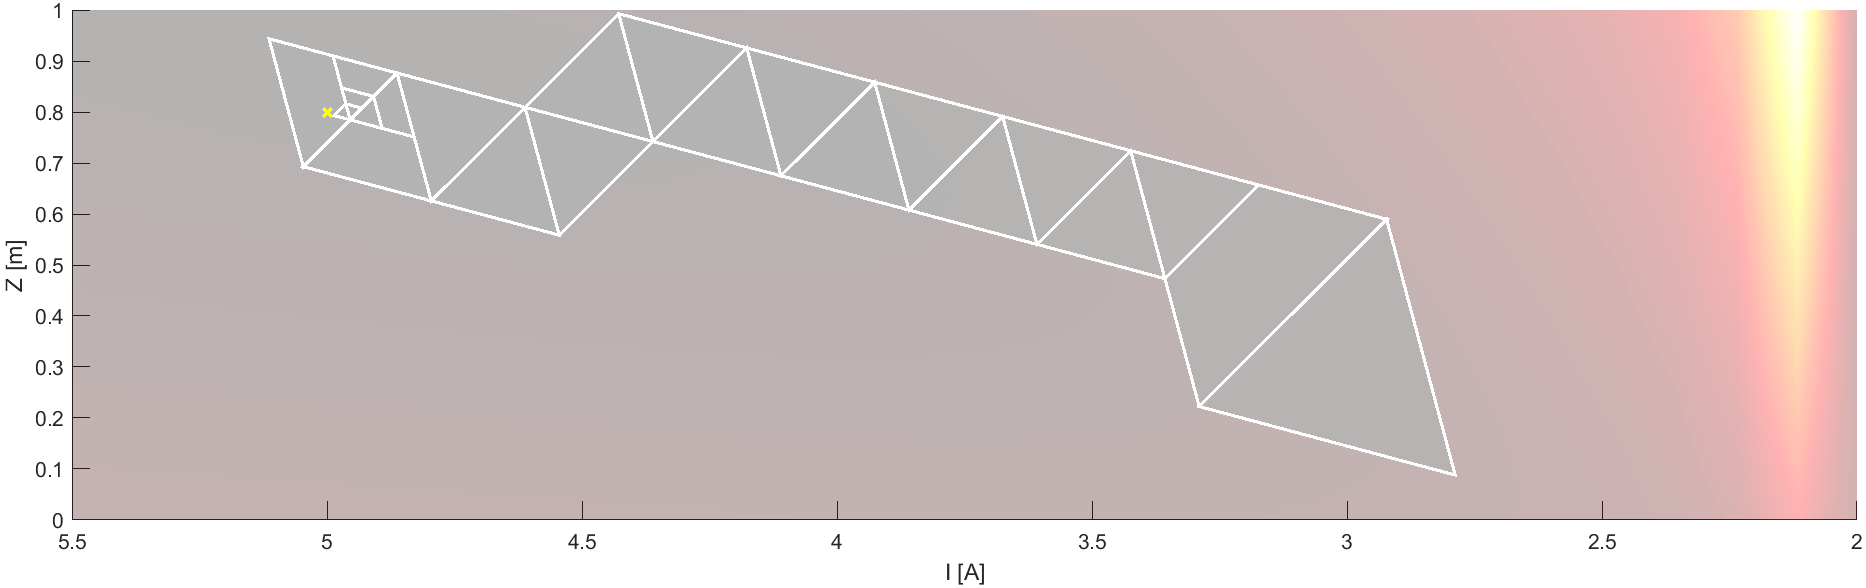
\includegraphics[width=15cm]{assets/figure10}
        \caption{Test con due gradi di libertà senza vincoli.}
\end{figure}

\section{Minimo in 3 dimensioni senza vincoli}

Proponiamo adesso dei test di ricerca del minimo non vincolato con 3 gradi di
libertà. Differentemente dal caso in due dimensioni, la percentuale di errore
aumenta all'aumentare del numero di campioni, a parità di percentuale di errore
massima.

\begin{table}[h]
    \caption{Test 3}
    \begin{center}
    \begin{tabular}{|l|l|l|l|} 
    \hline 
Gradi di libertà & \textbf{3} &  &  \\ \hline 
Passo & \textbf{0.100} & Campioni & \textbf{61} \\ \hline 
Punto di minimo & \textbf{{[}5.000 0.800 0.700{]}} & Punto di minimo &
\textbf{{[}4.953 0.791 0.699{]}} \\ \hline 
Punto iniziale & \textbf{{[}3.000 0.300 0.500{]}} & Fobj nel punto &
\textbf{0.00989} \\ \hline 
Lunghezza iniziale & \textbf{0.500} & Dimezzamenti & \textbf{7} \\ \hline 
Lunghezza minima & \textbf{0.00100} & Lunghezza finale & \textbf{0.00391} \\
\hline
Flip massimi & \textbf{1000} & Flips & \textbf{309} \\ \hline 
Tolleranza & \textbf{1.000\%} & \textbf{Perc. di errore} & \textbf{0.989\%} \\
\hline 
    \end{tabular}
    \end{center}
    \end{table}

    \begin{table}[h]
        \caption{Test}
        \begin{center}
        \begin{tabular}{|l|l|l|l|} 
        \hline 
        \multicolumn{2}{|c|}{\textbf{Parametri in ingresso}} & \multicolumn{2}{c|}{\textbf{Valori in uscita}} \\ \hline
        Gradi di libertà  & \textbf{3} &  &  \\ \hline 
        Passo & \textbf{0.100} & Campioni & \textbf{61} \\ \hline 
        Punto di minimo & \textbf{{[}5.000 0.800 0.700{]}} & Punto di minimo & \textbf{{[}4.999 0.799 0.700{]}} \\ \hline 
        Punto iniziale & \textbf{{[}3.000 0.300 0.500{]}} & Fobj nel punto & \textbf{0.00004} \\ \hline 
        Lunghezza iniziale & \textbf{0.500} & Dimezzamenti & \textbf{16} \\ \hline 
        Lunghezza minima & \textbf{0.00001} & Lunghezza finale & \textbf{0.00001} \\ \hline
        Flip massimi & \textbf{1000} & Flips & \textbf{654} \\ \hline 
        Tolleranza & \textbf{0.00100\%} & \textbf{Perc. di errore} & \textbf{0.00417\%} \\ \hline 
        \end{tabular}
        \end{center}
        \end{table}


\noindent
Abbassando la percentuale di errore ammissibile, miglioriamo i risultati
dell'algoritmo andando a raggiungere la lunghezza minima del lato del simplesso,
che noi facciamo coincidere con la massima risoluzione rispetto alla quale
valuteremo i parametri nello spazio di ricerca.

\begin{table}[h] 
    \caption{Test 4}
    \begin{center}
    \begin{tabular}{|l|l|l|l|} 
    \hline 
Gradi di libertà & \textbf{3} &  &  \\ \hline 
Passo & \textbf{0.100} & Campioni & \textbf{61} \\ \hline 
Punto di minimo & \textbf{{[}5.000 0.800 0.700{]}} & Punto di minimo &
\textbf{{[}4.981 0.796 0.699{]}} \\ \hline 
Punto iniziale & \textbf{{[}3.000 0.300 0.500{]}} & Fobj nel punto &
\textbf{0.00398} \\ \hline 
Lunghezza iniziale & \textbf{0.500} & Dimezzamenti & \textbf{9} \\ \hline 
Lunghezza minima & \textbf{0.00100} & Lunghezza finale & \textbf{0.000980} \\
\hline
Flip massimi & \textbf{1000} & Flips & \textbf{363} \\ \hline 
Tolleranza & \textbf{0.100\%} & \textbf{Perc. di errore} & \textbf{0.398\%} \\
\hline 
    \end{tabular} 
    \end{center}
    \end{table}

\noindent
Ripetendo gli stessi test con un passo di campionamento più fitto, si nota che
la percentuale di errore aumenta. Nel seguente test, la tolleranza $1\%$ causa
l'arresto dell'algoritmo.

\begin{table}[h] 
    \caption{Test 5}
    \begin{center}
    \begin{tabular}{|l|l|l|l|} 
    \hline 
Gradi di libertà & \textbf{3} &  &  \\ \hline 
Passo & \textbf{0.0100} & Campioni & \textbf{601} \\ \hline 
Punto di minimo & \textbf{{[}5.000 0.800 0.700{]}} & Punto di minimo &
\textbf{{[}4.954 0.789 0.698{]}} \\ \hline 
Punto iniziale & \textbf{{[}3.000 0.300 0.500{]}} & Fobj nel punto &
\textbf{0.00998} \\ \hline 
Lunghezza iniziale & \textbf{0.500} & Dimezzamenti & \textbf{6} \\ \hline 
Lunghezza minima & \textbf{0.00100} & Lunghezza finale & \textbf{0.00781} \\
\hline
Flip massimi & \textbf{1000} & Flips & \textbf{259} \\ \hline 
Tolleranza & \textbf{1.000\%} & \textbf{Perc. di errore} & \textbf{0.998\%} \\
\hline 
    \end{tabular} 
    \end{center}
    \end{table}

    \begin{table}[h]
        \caption{Test}
        \begin{center}
        \begin{tabular}{|l|l|l|l|} 
        \hline 
        \multicolumn{2}{|c|}{\textbf{Parametri in ingresso}} & \multicolumn{2}{c|}{\textbf{Valori in uscita}} \\ \hline
        Gradi di libertà  & \textbf{3} &  &  \\ \hline 
        Passo & \textbf{0.0100} & Campioni & \textbf{601} \\ \hline 
        Punto di minimo & \textbf{{[}5.000 0.800 0.700{]}} & Punto di minimo & \textbf{{[}4.999 0.799 0.700{]}} \\ \hline 
        Punto iniziale & \textbf{{[}3.000 0.300 0.500{]}} & Fobj nel punto & \textbf{0.00002} \\ \hline 
        Lunghezza iniziale & \textbf{0.500} & Dimezzamenti & \textbf{16} \\ \hline 
        Lunghezza minima & \textbf{0.00001} & Lunghezza finale & \textbf{0.00001} \\ \hline
        Flip massimi & \textbf{1000} & Flips & \textbf{709} \\ \hline 
        Tolleranza & \textbf{0.00100\%} & \textbf{Perc. di errore} & \textbf{0.00205\%} \\ \hline 
        \end{tabular}
        \end{center}
        \end{table}
\noindent
Abbassando la percentuale di errore, si nota che l'algoritmo si ferma a causa
della lunghezza finale del lato del simplesso troppo bassa. Questa è una
conseguenza del fatto che, avendo aumentato la risoluzione con il passo di
campionamento più fitto, la funziona sarà a sua volta più definita e quindi
l'algoritmo si troverà con più probabilità in situazioni dove il dimezzamento è
necessario.

\begin{table}[h] 
    \caption{Test 6}
    \begin{center}
    \begin{tabular}{|l|l|l|l|} 
    \hline 
Gradi di libertà & \textbf{3} &  &  \\ \hline 
Passo & \textbf{0.01000} & Campioni & \textbf{601} \\ \hline 
Punto di minimo & \textbf{{[}5.000 0.800 0.700{]}} & Punto di minimo &
\textbf{{[}4.968 0.794 0.699{]}} \\ \hline 
Punto iniziale & \textbf{{[}3.000 0.300 0.500{]}} & Fobj nel punto &
\textbf{0.00651} \\ \hline 
Lunghezza iniziale & \textbf{0.500} & Dimezzamenti & \textbf{9} \\ \hline 
Lunghezza minima & \textbf{0.00100} & Lunghezza finale & \textbf{0.000980} \\
\hline
Flip massimi & \textbf{1000} & Flips & \textbf{309} \\ \hline 
Tolleranza & \textbf{0.100\%} & \textbf{Perc. di errore} & \textbf{0.651\%} \\
\hline 
    \end{tabular}
    \end{center}
    \end{table}

\begin{figure}[H]
    \centering
        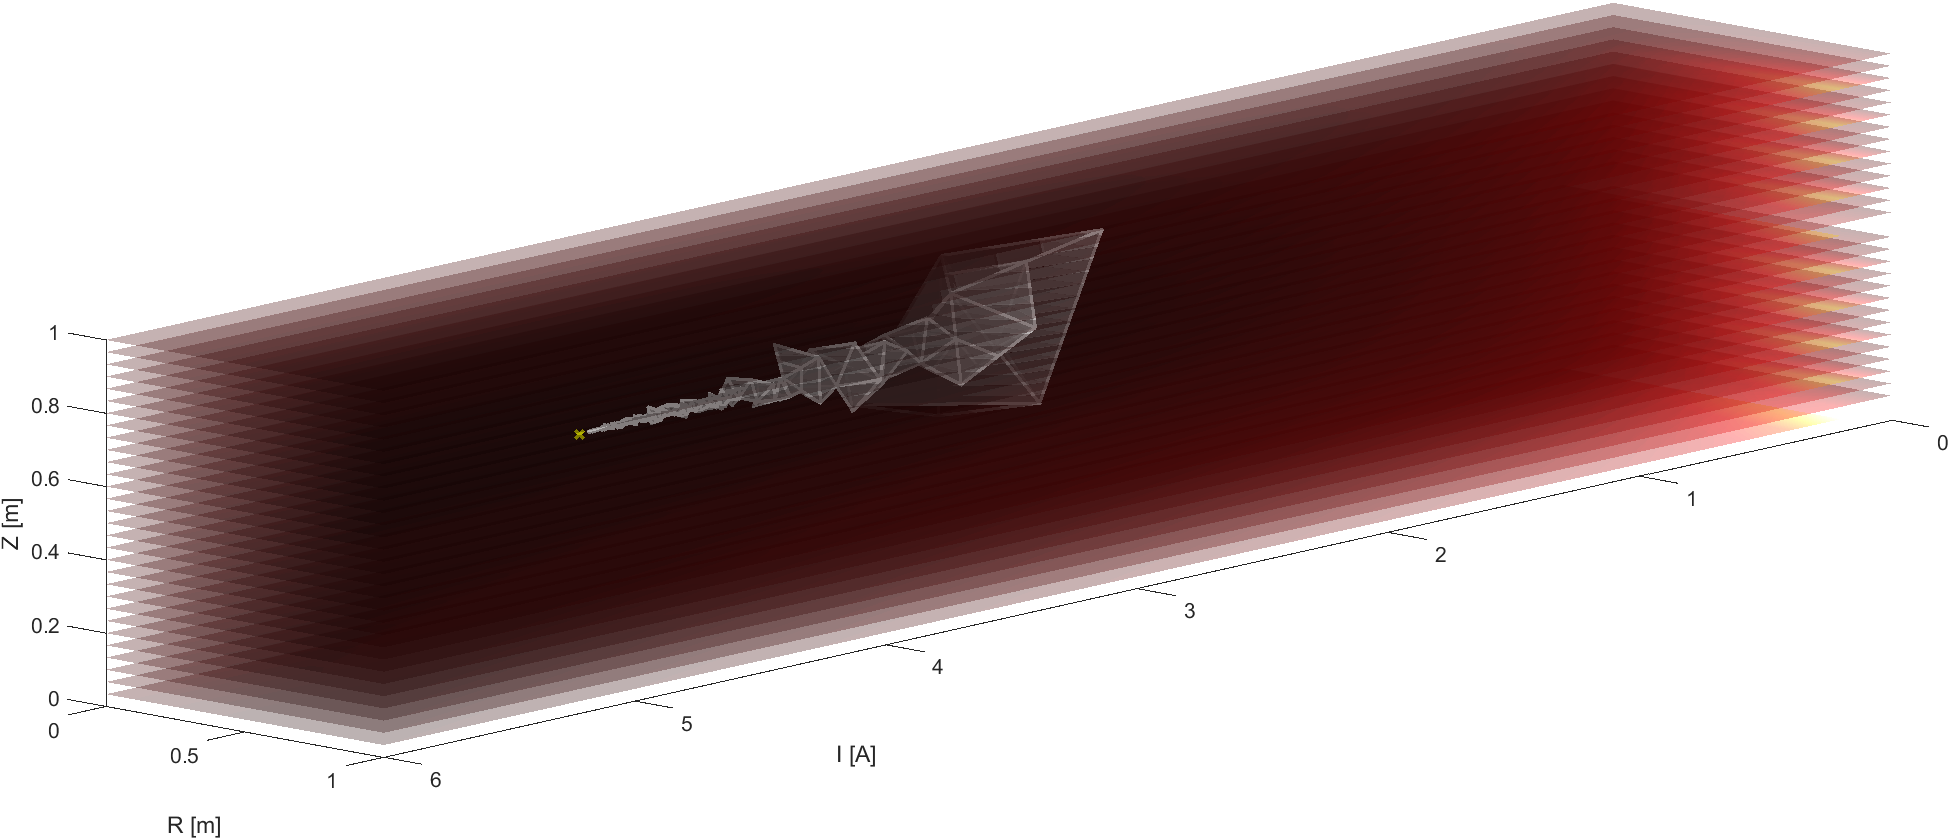
\includegraphics[width=16cm]{assets/figure4}
        \caption{Ricerca del minimo non vincolato con 3 parametri liberi, test 5.}
\end{figure}
\noindent 

\begin{figure}[H]
    \centering
        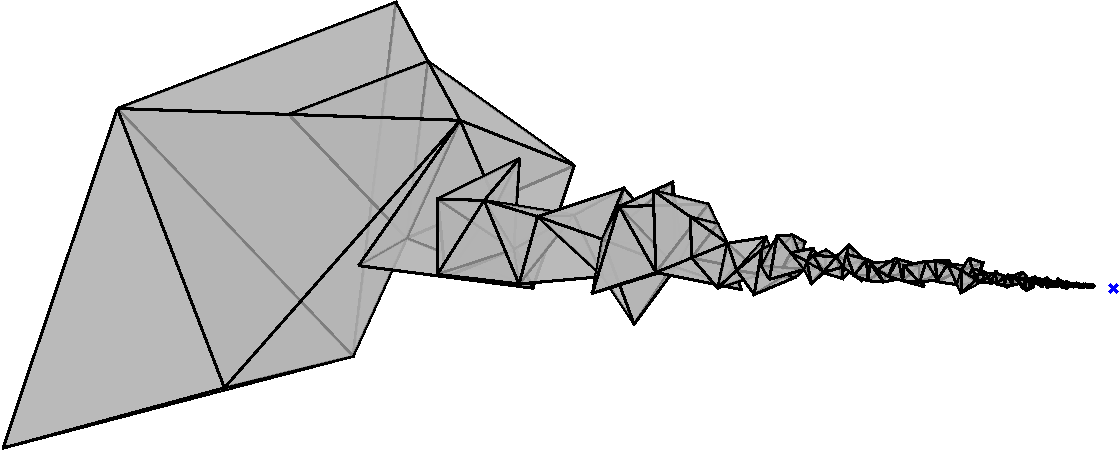
\includegraphics[width=14cm]{assets/figure5}
        \caption{Dettaglio del politopo generato al test 5.}
\end{figure}
\noindent 

\begin{figure}[H]
    \centering
        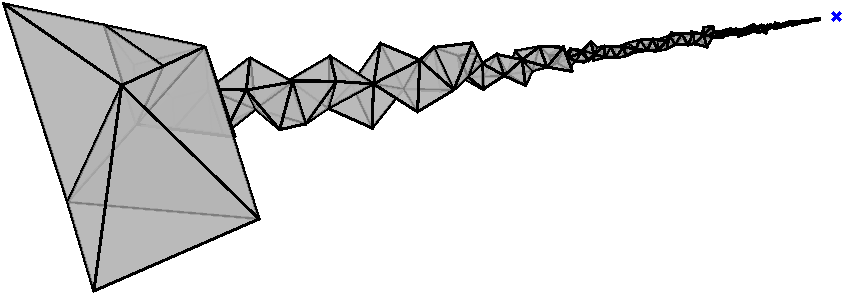
\includegraphics[width=14cm]{assets/figure6}
        \caption{Dettaglio del politopo generato al test 5.}
\end{figure}
\noindent

\newpage
\section{Minimo in 3 dimensioni con vincolo di disuguaglianza}

Effettuiamo un test per verificare il corretto funzionamento dell'algoritmo e
appurarne le prestazioni in presenza di un vincolo di disuguaglianza $R \le 2Z$.
\\
Il vincolo di disuguaglianza è stato trattato algoritmicamente con la tecnica
delle \emph{penalità}, in modo tale da rendere molto alto il valore della
funzione obiettivo valutato nei vertici del simplesso oltrepassanti il vincolo
(mediante un fattore moltiplicativo $p = 100$). \\
Come si evince dai due test effettuati con gli stessi parametri ma con un punto
iniziale diverso, è evidente che i risultati sono anche molto diversi a seconda
del punto.

\begin{table}[h]
    \caption{Test 7}
    \begin{center}
    \begin{tabular}{|l|l|l|l|} 
    \hline 
Gradi di libertà & \textbf{3} &  &  \\ \hline 
Passo & \textbf{0.100} &  &  \\ \hline 
Punto di minimo & \textbf{{[}5.000 0.800 0.700{]}} & Punto di minimo &
\textbf{{[}4.093 0.991 0.495{]}} \\ \hline 
Punto iniziale & \textbf{{[}4.000 0.400 0.100{]}} & Fobj nel punto &
\textbf{0.320} \\ \hline 
Lunghezza iniziale & \textbf{0.500} & Dimezzamenti & \textbf{9} \\ \hline 
Lunghezza minima & \textbf{0.00100} & Lunghezza finale & \textbf{0.000980} \\
\hline
Flip massimi & \textbf{1000} & Flips & \textbf{104} \\ \hline 
Tolleranza & \textbf{1.000\%} & \textbf{Perc. di errore} & \textbf{32.012\%} \\
\hline 
    \end{tabular} 
    \end{center}
    \end{table}

\begin{figure}[H]
    \centering
        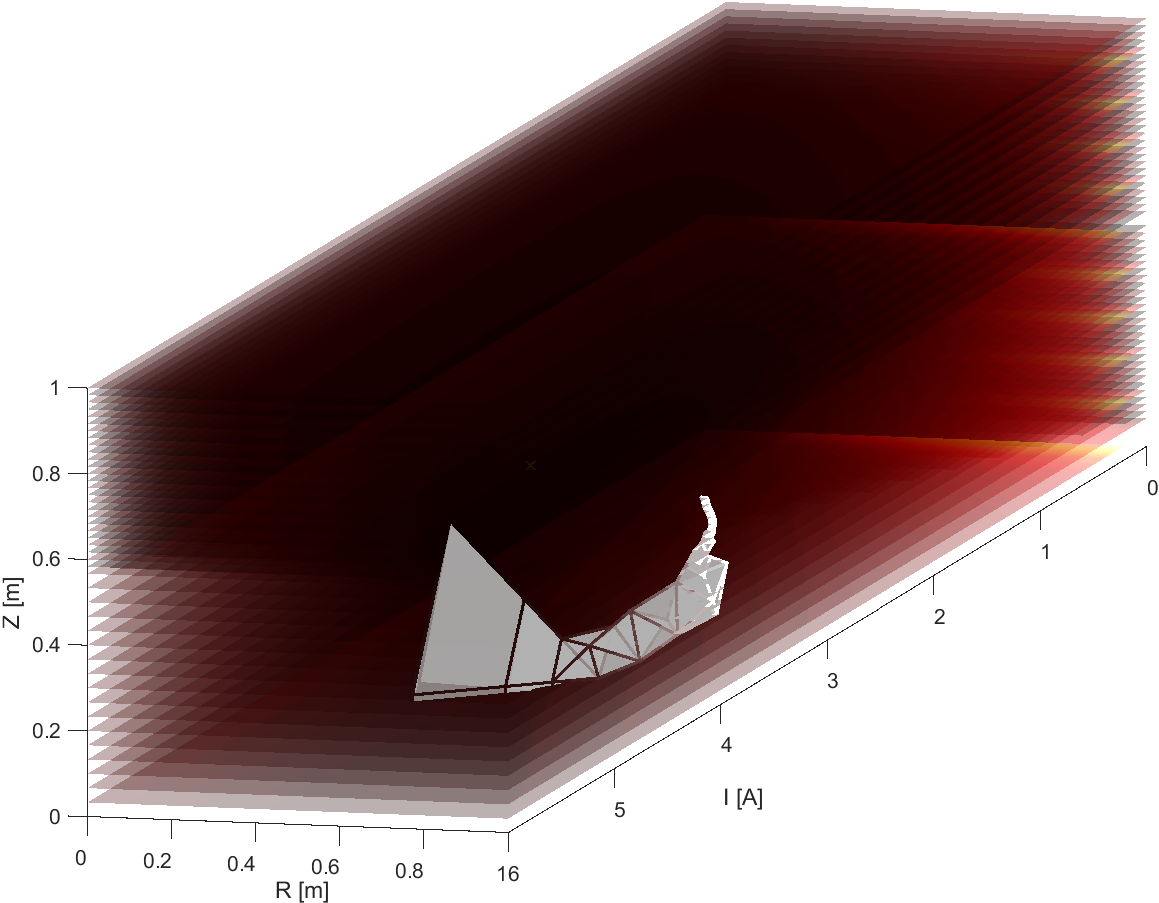
\includegraphics[width=14cm]{assets/figure7}
        \caption{Test con vincolo attivo di disuguaglianza.}
\end{figure}
\noindent

\begin{table}[h]
    \caption{Test 8}
    \begin{center}
    \begin{tabular}{|l|l|l|l|} 
    \hline 
Gradi di libertà & \textbf{3} &  &  \\ \hline 
Passo & \textbf{0.100} &  &  \\ \hline 
Punto di minimo & \textbf{{[}5.000 0.800 0.700{]}} & Punto di minimo &
\textbf{{[}3.406 0.885 0.442{]}} \\ \hline 
Punto iniziale & \textbf{{[}3.000 0.400 0.100{]}} & Fobj nel punto &
\textbf{0.449} \\ \hline 
Lunghezza iniziale & \textbf{0.500} & Dimezzamenti & \textbf{9} \\ \hline 
Lunghezza minima & \textbf{0.00100} & Lunghezza finale & \textbf{0.000980} \\
\hline
Flip massimi & \textbf{1000} & Flips & \textbf{122} \\ \hline 
Tolleranza & \textbf{1.000\%} & \textbf{Perc. di errore} & \textbf{44.908\%} \\
\hline 
    \end{tabular}
    \end{center}
    \end{table}

\begin{figure}[H]
    \centering
        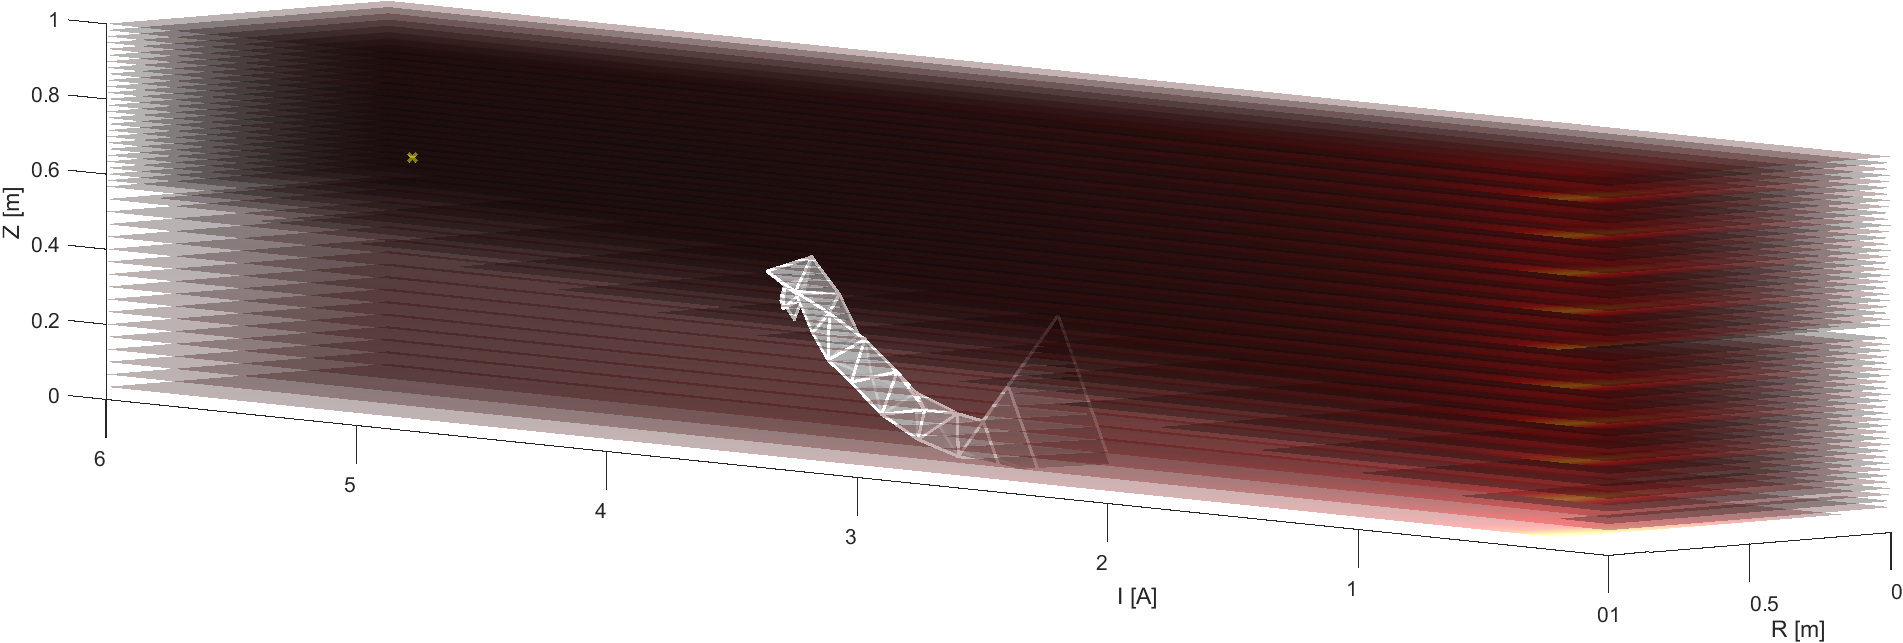
\includegraphics[width=16cm]{assets/figure8}
        \caption{Test con vincolo attivo di disuguaglianza.}
\end{figure}
\noindent

\begin{figure}[H]
    \centering
        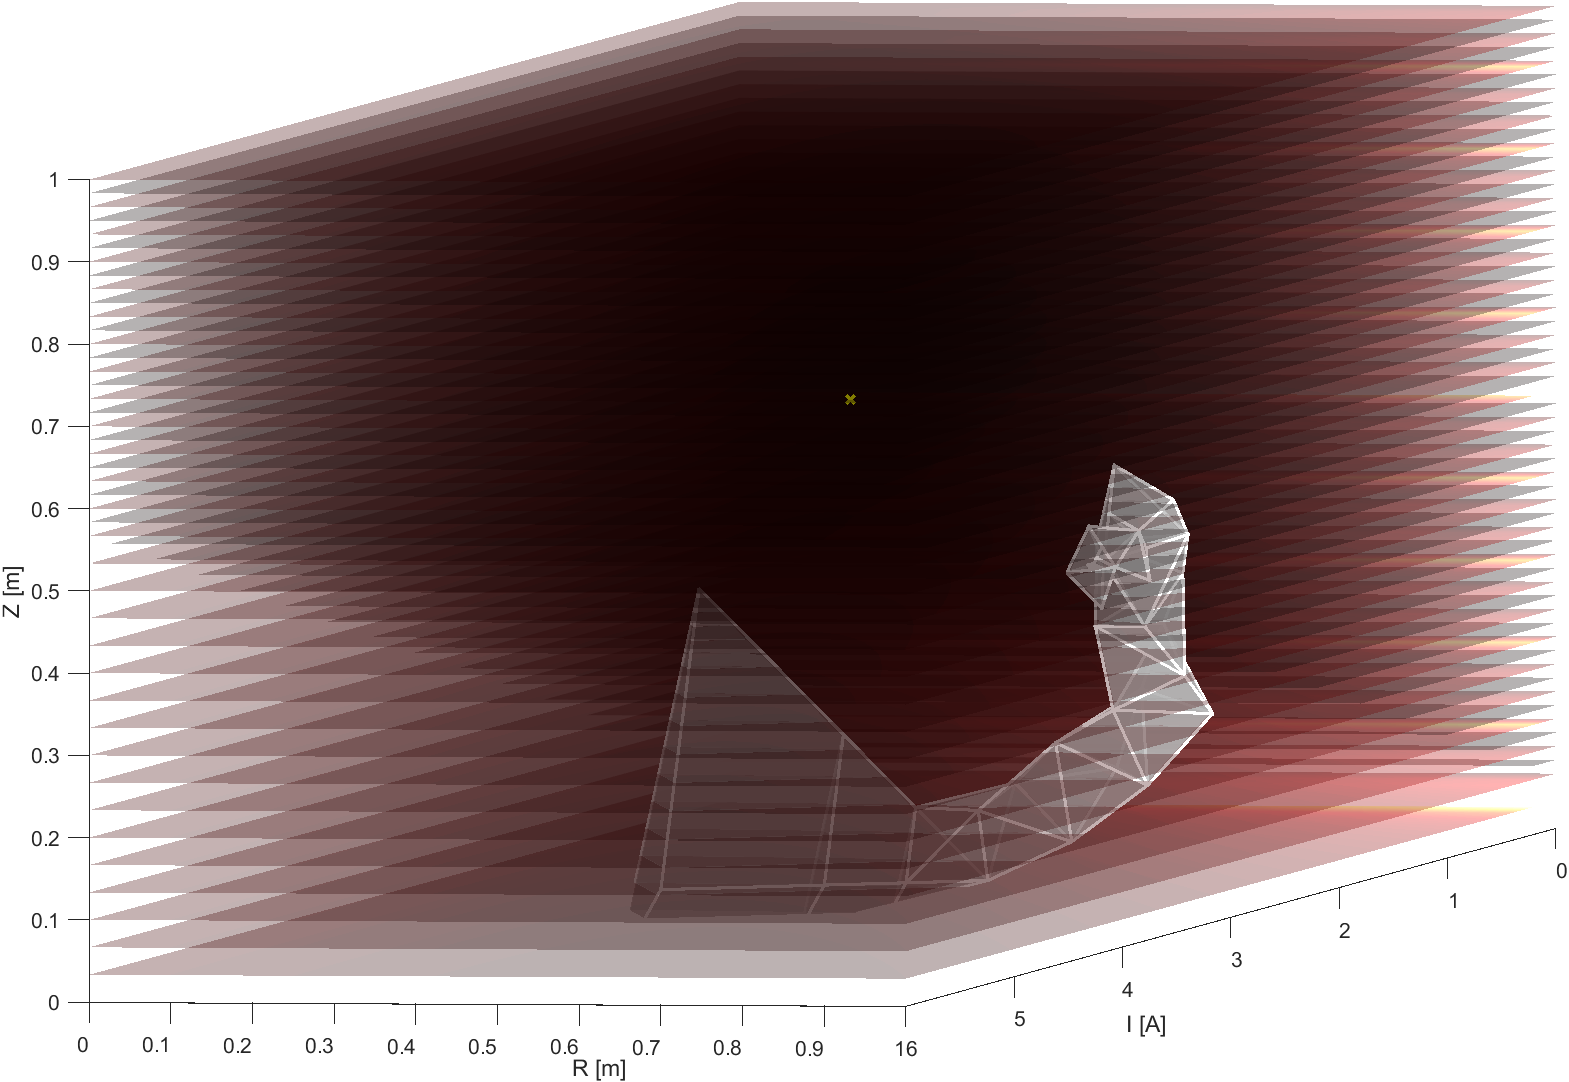
\includegraphics[width=13cm]{assets/figure9}
        \caption{Test con vincolo attivo di disuguaglianza.}
\end{figure}

\newpage
\section{Minimo in 2 dimensioni: vincolo di uguaglianza}

I seguenti test sono stati effettuati applicando il vincolo di uguaglianza $R =
2Z$. Da considerare inoltre che verranno tenuti in considerazione i vincoli di
progetto imposti a priori, ovvero $R \le 1m$ e $Z \le 1m$. Siccome vale il
vincolo descritto precedentemente, il valore di $Z$ non potrà essere superiore a
$0.5m$ altrimenti la ricerca comporterebbe risultati che non sono compatibili
con i limiti progettuali imposti. \\
Le prove effettuate con diversi parametri (ma stesso punto iniziale) portano
agli stessi risultati in termine di percentuale di errore dalla funzione
desiderata.

\begin{table}[h]
    \caption{Test 9 - Incognite $I$ e $Z$}
    \begin{center}
    \begin{tabular}{|l|l|l|l|} 
    \hline 
Gradi di libertà & \textbf{2} &  &  \\ \hline 
Passo & \textbf{0.100} & Campioni & \textbf{61} \\ \hline 
Punto di minimo & \textbf{{[}5.000 0.700{]}} & Punto di minimo &
\textbf{{[}4.097 0.998 0.499{]}} \\ \hline 
Punto iniziale & \textbf{{[}3.000 0.300{]}} & Fobj nel punto & \textbf{0.354} \\
\hline 
Lunghezza iniziale & \textbf{0.200} & Dimezzamenti & \textbf{9} \\ \hline 
Lunghezza minima & \textbf{0.00100} & Lunghezza finale & \textbf{0.000680} \\
\hline
Flip massimi & \textbf{1000} & Flips & \textbf{151} \\ \hline 
Tolleranza & \textbf{1.000\%} & \textbf{Perc. di errore} & \textbf{35.355\%} \\
\hline 
    \end{tabular} 
    \end{center}
    \end{table}




\begin{figure}[H]
    \centering
        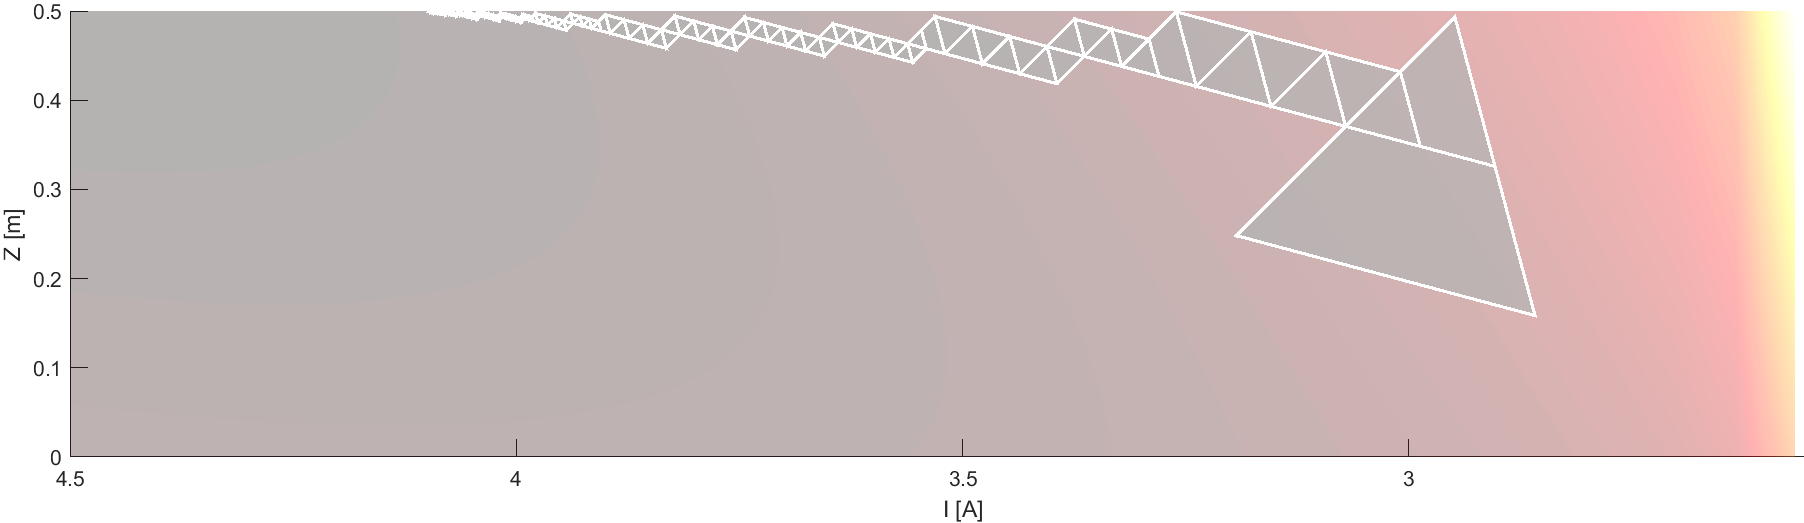
\includegraphics[width=15cm]{assets/figure11}
        \caption{Test con vincolo di uguaglianza.}
\end{figure}

\newpage
\section*{Risultati e considerazioni}




\begin{figure}[H]
    \centering
        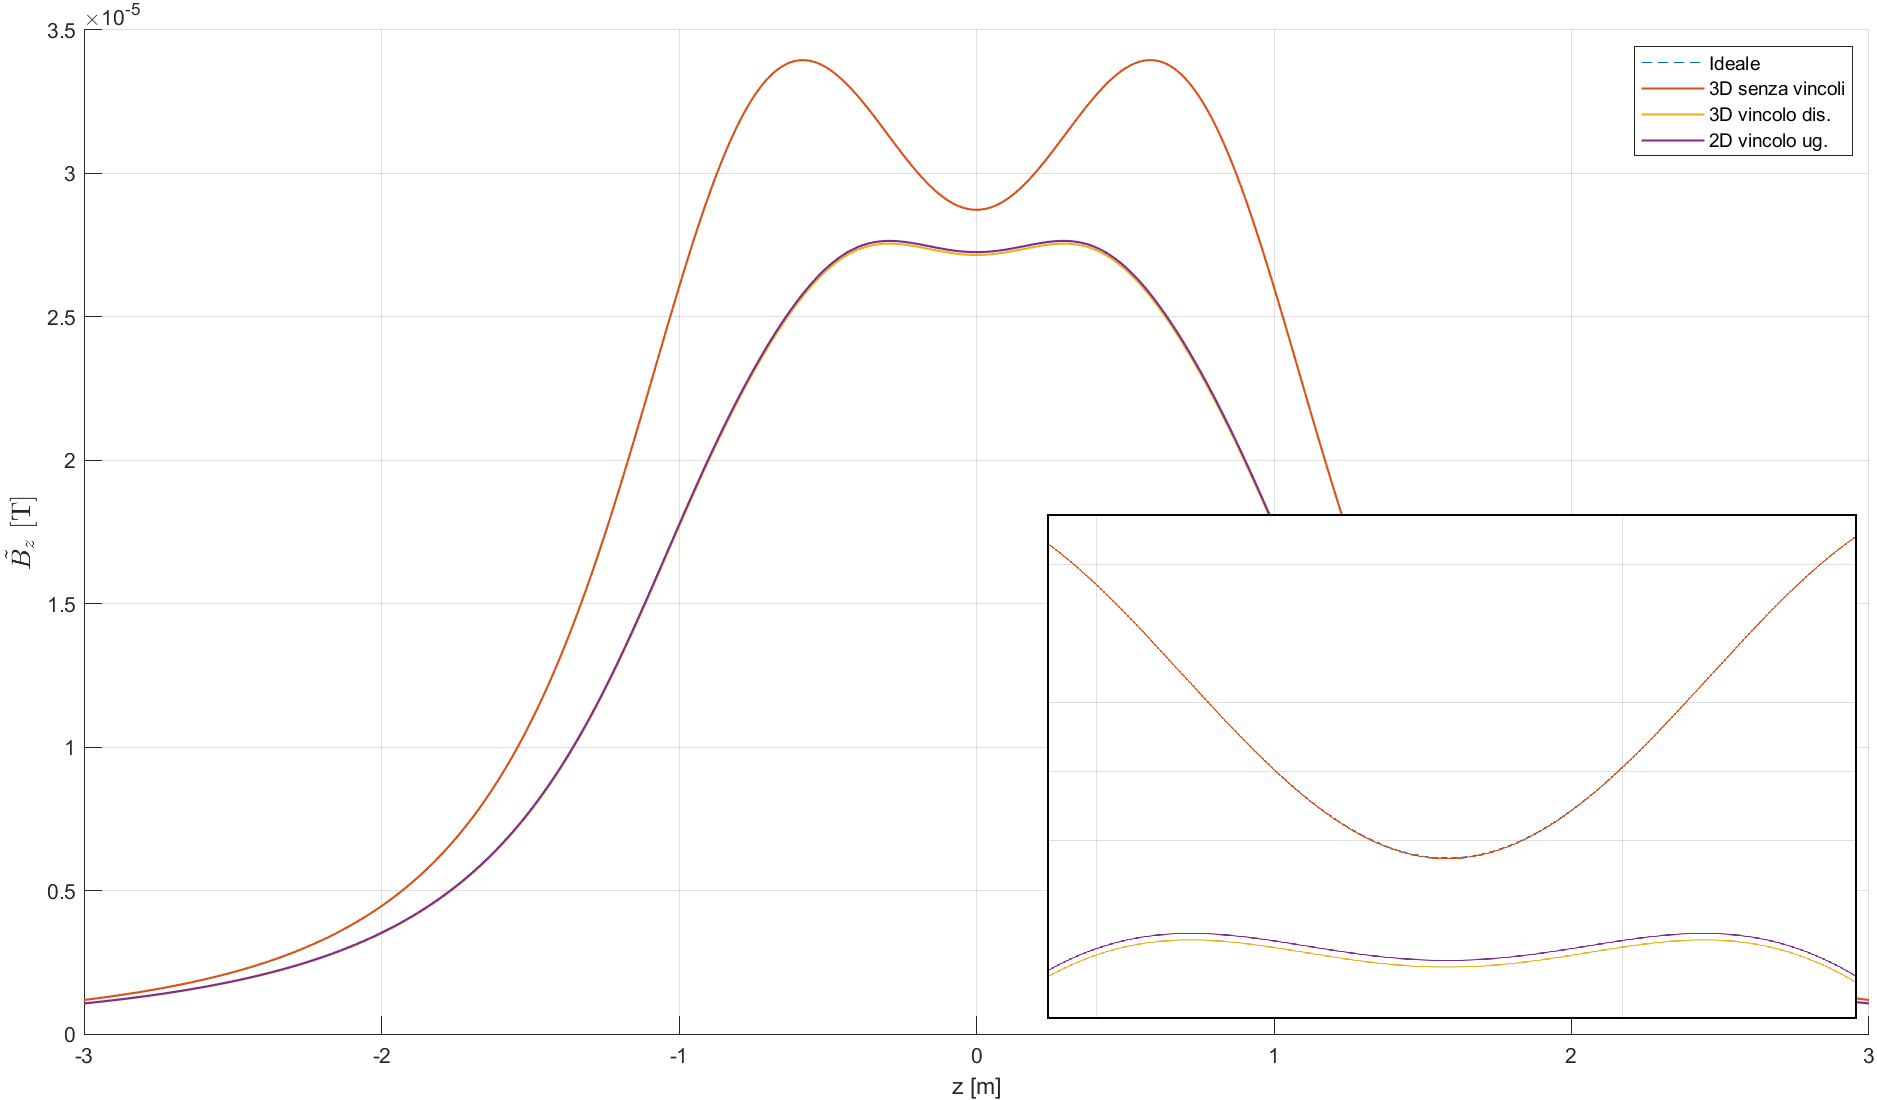
\includegraphics[width=16cm]{assets/figure12}
        \caption{Confronto dei risultati ottenuti.}
\end{figure}

I risultati ottenuti dai test provano una solida implementazione dell'algoritmo
del simplesso per la ricerca del minimo di una funzione di costo. \\
Per tutti i risultati commentati a seguire, si è scelto di assumere una
precisione della \emph{terza cifra decimale}. La motivazione risiede nel
fatto che, per limiti di realizzazione fisica delle spire, non riusciremo a
garantire una precisione maggiore del millimetro per il raggio della spira
incognita. \\ 
Inoltre, siccome il minimo spostamento del simplesso nello spazio di ricerca
sarà proprio vincolato da questo limite realizzativo, anche la precisione delle
altre due variabili incognite si fermerà alla terza cifra decimale. \\ \\
Nel test preliminare con due gradi di libertà, il punto di minimo ottenuto
risulta essere \\ \\
\centerline{ $I_{2} = 4.998 \pm 0.001 A$ \\ $R_{2} = 0.800 \pm 0.001m$ \\ $Z_{2}
= 0.7m$} \\ \\
con rispetto ai parametri iniziali e le condizioni di arresto scelte.
L'algoritmo si è fermato dopo 90 ribaltamenti e 7 dimezzamenti, a causa della
percentuale di errore scesa sotto la soglia che abbiamo ritenuto sufficiente
all'avvio della computazione. Se la percentuale di errore massima fosse stata
minore, i risultati ottenuti sarebbero potuti essere ancora migliori. \\
\\
L'esperimento effettuato in uno spazio di ricerca tridimensionale senza vincoli
ha dato dei risultati inattesi, in quanto ci si aspettava che la precisione
migliorasse all'aumentare del numero di campioni della funzione obiettivo. \\
Il motivo per il quale invece le prestazioni sono state migliori in presenza di
meno campioni è quello della scelta delle condizioni di arresto.
Nell'esperimento con $601$ campioni, infatti, la funzione risulta essere più
definita. Ciò ha comportato quindi anche una valutazione più accurata della
funzione obiettivo ai vertici del simplesso, che con più probabilità si è
ritrovato in una condizione di flip continuo tra gli stessi vertici, causando
invecchiamento di un pivot e quindi dimezzamento, con conseguente riduzione
della lunghezza del lato del simplesso (vincolo di arresto). \\
Siccome la lunghezza minima del lato del simplesso è stata fissata al minimo
scostamento apprezzabile in fase di realizzazione dei componenti fisici del
sistema da analizzare, l'aver raggiunto più velocemente questa condizione ha
comportato dei risultati più grossolani di quanto ci si aspettava. Se i limiti
di realizzazione delle componenti fisiche fossero stati più spinti, l'algoritmo
sarebbe andato più in fondo e avrebbe garantito dei risultati paragonabili in
qualità a quelli ottenuti nel caso in due dimensioni visto precedentemente. Il
punto di minimo ottenuto quindi nell'esperimento con 3 gradi di libertà senza
vincoli è \\ \\
\centerline{ $I_{2} = 4.981 \pm 0.001 A$ \\ $R_{2} = 0.796 \pm 0.001m$ \\ $Z_{2}
= 0.699 \pm 0.001m$} \\ \\
Nel caso della ricerca del minimo in 3D con vincolo di disuguaglianza invece,
evince chiaramente l'importanza della scelta del punto iniziale. Cambiando il
punto negli esperimenti effettuati, infatti, si possono anche avere discrepanze
di 10 punti percentuali rispetto all'errore ottenuto nelle stesse condizioni, ma
punto iniziale diverso. Il punto di minimo ottenuto in questo caso è \\ \\
\centerline{ $I_{2} = 4.093 \pm 0.001 A$ \\ $R_{2} = 0.991 \pm 0.001m$ \\ $Z_{2}
= 0.495 \pm 0.001m$} \\ \\
Il quarto ed ultimo esperimento si è invece concentrato sulla ricerca del minimo
in presenza di un vincolo di uguaglianza, che fa ridurre la dimensione dello
spazio di ricerca da 3 a 2. Con i parametri iniziali e le condizioni di arresto
scelte, si ottiene un punto di minimo di \\ \\
\centerline{ $I_{2} = 4.097 \pm 0.001 A$ \\ $R_{2} = 0.998 \pm 0.001m$ \\ $Z_{2}
= 0.499 \pm 0.001m$} \\ \\
Di particolare interesse è stata l'applicazione dei limiti di progetto
preliminari imposti ad inizio trattazione. \\ 
Siccome nè raggio nè posizione della spira possono oltrepassare la lunghezza di
$1m$, questa condizione combinata al vincolo di uguaglianza $R = 2Z$ comporta la
scelta di valori accettabili per la $Z$ fino a $0.5m$. L'esperimento ha
confermato i risultati aspettati, in quanto il valore ideale della posizione
della spira incognita è maggiore del massimo imposto dai vincoli realizzativi. È
quindi chiaro che l'algoritmo tende a muoversi verso la direzione del minimo
ideale fino a raggiungere il valore massimo ammissibile della $Z = 0.5m$.





\end{document}




